\batchmode
\documentclass[twoside]{book}

% Packages required by doxygen
\usepackage{fixltx2e}
\usepackage{calc}
\usepackage{doxygen}
\usepackage[export]{adjustbox} % also loads graphicx
\usepackage{graphicx}
\usepackage[utf8]{inputenc}
\usepackage{makeidx}
\usepackage{multicol}
\usepackage{multirow}
\PassOptionsToPackage{warn}{textcomp}
\usepackage{textcomp}
\usepackage[nointegrals]{wasysym}
\usepackage[table]{xcolor}

% Font selection
\usepackage[T1]{fontenc}
\usepackage[scaled=.90]{helvet}
\usepackage{courier}
\usepackage{amssymb}
\usepackage{sectsty}
\renewcommand{\familydefault}{\sfdefault}
\allsectionsfont{%
  \fontseries{bc}\selectfont%
  \color{darkgray}%
}
\renewcommand{\DoxyLabelFont}{%
  \fontseries{bc}\selectfont%
  \color{darkgray}%
}
\newcommand{\+}{\discretionary{\mbox{\scriptsize$\hookleftarrow$}}{}{}}

% Page & text layout
\usepackage{geometry}
\geometry{%
  a4paper,%
  top=2.5cm,%
  bottom=2.5cm,%
  left=2.5cm,%
  right=2.5cm%
}
\tolerance=750
\hfuzz=15pt
\hbadness=750
\setlength{\emergencystretch}{15pt}
\setlength{\parindent}{0cm}
\setlength{\parskip}{3ex plus 2ex minus 2ex}
\makeatletter
\renewcommand{\paragraph}{%
  \@startsection{paragraph}{4}{0ex}{-1.0ex}{1.0ex}{%
    \normalfont\normalsize\bfseries\SS@parafont%
  }%
}
\renewcommand{\subparagraph}{%
  \@startsection{subparagraph}{5}{0ex}{-1.0ex}{1.0ex}{%
    \normalfont\normalsize\bfseries\SS@subparafont%
  }%
}
\makeatother

% Headers & footers
\usepackage{fancyhdr}
\pagestyle{fancyplain}
\fancyhead[LE]{\fancyplain{}{\bfseries\thepage}}
\fancyhead[CE]{\fancyplain{}{}}
\fancyhead[RE]{\fancyplain{}{\bfseries\leftmark}}
\fancyhead[LO]{\fancyplain{}{\bfseries\rightmark}}
\fancyhead[CO]{\fancyplain{}{}}
\fancyhead[RO]{\fancyplain{}{\bfseries\thepage}}
\fancyfoot[LE]{\fancyplain{}{}}
\fancyfoot[CE]{\fancyplain{}{}}
\fancyfoot[RE]{\fancyplain{}{\bfseries\scriptsize Generated by Doxygen }}
\fancyfoot[LO]{\fancyplain{}{\bfseries\scriptsize Generated by Doxygen }}
\fancyfoot[CO]{\fancyplain{}{}}
\fancyfoot[RO]{\fancyplain{}{}}
\renewcommand{\footrulewidth}{0.4pt}
\renewcommand{\chaptermark}[1]{%
  \markboth{#1}{}%
}
\renewcommand{\sectionmark}[1]{%
  \markright{\thesection\ #1}%
}

% Indices & bibliography
\usepackage{natbib}
\usepackage[titles]{tocloft}
\setcounter{tocdepth}{3}
\setcounter{secnumdepth}{5}
\makeindex

% Hyperlinks (required, but should be loaded last)
\usepackage{ifpdf}
\ifpdf
  \usepackage[pdftex,pagebackref=true]{hyperref}
\else
  \usepackage[ps2pdf,pagebackref=true]{hyperref}
\fi
\hypersetup{%
  colorlinks=true,%
  linkcolor=blue,%
  citecolor=blue,%
  unicode%
}

% Custom commands
\newcommand{\clearemptydoublepage}{%
  \newpage{\pagestyle{empty}\cleardoublepage}%
}

\usepackage{caption}
\captionsetup{labelsep=space,justification=centering,font={bf},singlelinecheck=off,skip=4pt,position=top}

%===== C O N T E N T S =====

\begin{document}

% Titlepage & ToC
\hypersetup{pageanchor=false,
             bookmarksnumbered=true,
             pdfencoding=unicode
            }
\pagenumbering{alph}
\pagenumbering{arabic}
\hypersetup{pageanchor=true}

%--- Begin generated contents ---
\chapter{Example problem\+: Finite-\/\+Reynolds-\/number flow inside an oscillating ellipse}
\label{index}\hypertarget{index}{}\hypertarget{index_q}{}\section{A few quick questions...}\label{index_q}
Since {\ttfamily oomph-\/lib} is developed as open-\/source software, any evidence that the code is being downloaded and used is very helpful for us as it helps to justify our continued work on this project.

We would therefore be extremely grateful if you could provide the information requested in the form below. Pressing the \char`\"{}submit\char`\"{} button will get you to the actual download page.

{\bfseries Note\+:} 
\begin{DoxyItemize}
\item All information will be treated as confidential. 
\item If you provide your email address and check the appropriate box we will add you to our mailing list to inform you of upgrades and bug fixes to the code. Rest assured that the mailing list is {\bfseries very low volume} -- we have better things to do than to bombard you with email. 
\item If you still feel reluctant to provide any of the information requested, feel free to enter some dummy input. The form will check that {\bfseries some} information has been entered but entering your name as \char`\"{}\+Joe Cool\char`\"{} is perfectly acceptable -- this is to discourage people from not providing the information simply because they are too lazy to type... 
\end{DoxyItemize}



 







 

 \hypertarget{index_pdf}{}\section{P\+D\+F file}\label{index_pdf}
A \href{../latex/refman.pdf}{\tt pdf version} of this document is available. \end{document}

\chapter{Namespace Index}
\section{Namespace List}
Here is a list of all namespaces with brief descriptions\+:\begin{DoxyCompactList}
\item\contentsline{section}{\hyperlink{namespaceGlobal__Physical__Variables}{Global\+\_\+\+Physical\+\_\+\+Variables} \\*Global variables that represent physical properties }{\pageref{namespaceGlobal__Physical__Variables}}{}
\item\contentsline{section}{\hyperlink{namespaceoomph}{oomph} }{\pageref{namespaceoomph}}{}
\item\contentsline{section}{\hyperlink{namespacePhysical__Variables}{Physical\+\_\+\+Variables} \\*Namespace for the solution of 2D linear shell equation }{\pageref{namespacePhysical__Variables}}{}
\end{DoxyCompactList}

\chapter{Hierarchical Index}
\section{Class Hierarchy}
This inheritance list is sorted roughly, but not completely, alphabetically\+:\begin{DoxyCompactList}
\item Problem\begin{DoxyCompactList}
\item \contentsline{section}{Unstructured\+Solid\+Problem$<$ E\+L\+E\+M\+E\+NT $>$}{\pageref{classUnstructuredSolidProblem}}{}
\end{DoxyCompactList}
\end{DoxyCompactList}

\chapter{Class Index}
\section{Class List}
Here are the classes, structs, unions and interfaces with brief descriptions\+:\begin{DoxyCompactList}
\item\contentsline{section}{\hyperlink{classPMLProblem}{P\+M\+L\+Problem$<$ E\+L\+E\+M\+E\+N\+T $>$} }{\pageref{classPMLProblem}}{}
\item\contentsline{section}{\hyperlink{classGlobalParameters_1_1TestPMLMapping}{Global\+Parameters\+::\+Test\+P\+M\+L\+Mapping} }{\pageref{classGlobalParameters_1_1TestPMLMapping}}{}
\end{DoxyCompactList}

\chapter{File Index}
\section{File List}
Here is a list of all files with brief descriptions\+:\begin{DoxyCompactList}
\item\contentsline{section}{\hyperlink{jeffery__orbit_8cc}{jeffery\+\_\+orbit.\+cc} }{\pageref{jeffery__orbit_8cc}}{}
\item\contentsline{section}{\hyperlink{jeffery__orbit_8txt__doxygenified_8h}{jeffery\+\_\+orbit.\+txt\+\_\+doxygenified.\+h} }{\pageref{jeffery__orbit_8txt__doxygenified_8h}}{}
\item\contentsline{section}{\hyperlink{my__taylor__hood__elements_8h}{my\+\_\+taylor\+\_\+hood\+\_\+elements.\+h} }{\pageref{my__taylor__hood__elements_8h}}{}
\end{DoxyCompactList}

\chapter{Namespace Documentation}
\hypertarget{namespaceGlobal__Physical__Variables}{}\section{Global\+\_\+\+Physical\+\_\+\+Variables Namespace Reference}
\label{namespaceGlobal__Physical__Variables}\index{Global\+\_\+\+Physical\+\_\+\+Variables@{Global\+\_\+\+Physical\+\_\+\+Variables}}


Namespace for physical parameters.  


\subsection*{Functions}
\begin{DoxyCompactItemize}
\item 
Vector$<$ double $>$ \hyperlink{namespaceGlobal__Physical__Variables_afae321364975eb56688ad13abc8ed6b7}{Gravity} (2)
\begin{DoxyCompactList}\small\item\em Gravity vector. \end{DoxyCompactList}\item 
void \hyperlink{namespaceGlobal__Physical__Variables_a87da705b8a46bed337cf5dbdd788b87b}{body\+\_\+force} (const double \&time, const Vector$<$ double $>$ \&x, Vector$<$ double $>$ \&result)
\begin{DoxyCompactList}\small\item\em Functional body force. \end{DoxyCompactList}\item 
void \hyperlink{namespaceGlobal__Physical__Variables_a9780d615ae07c4e00a436ab2973b54e6}{zero\+\_\+body\+\_\+force} (const double \&time, const Vector$<$ double $>$ \&x, Vector$<$ double $>$ \&result)
\begin{DoxyCompactList}\small\item\em Zero functional body force. \end{DoxyCompactList}\end{DoxyCompactItemize}
\subsection*{Variables}
\begin{DoxyCompactItemize}
\item 
double \hyperlink{namespaceGlobal__Physical__Variables_ab814e627d2eb5bc50318879d19ab16b9}{Re} =100
\begin{DoxyCompactList}\small\item\em Reynolds number. \end{DoxyCompactList}\item 
double \hyperlink{namespaceGlobal__Physical__Variables_ab1a845a672b4d74b304639a976dc65c6}{Re\+\_\+inv\+Fr} =100
\begin{DoxyCompactList}\small\item\em Reynolds/\+Froude number. \end{DoxyCompactList}\end{DoxyCompactItemize}


\subsection{Detailed Description}
Namespace for physical parameters. 

\subsection{Function Documentation}
\mbox{\Hypertarget{namespaceGlobal__Physical__Variables_a87da705b8a46bed337cf5dbdd788b87b}\label{namespaceGlobal__Physical__Variables_a87da705b8a46bed337cf5dbdd788b87b}} 
\index{Global\+\_\+\+Physical\+\_\+\+Variables@{Global\+\_\+\+Physical\+\_\+\+Variables}!body\+\_\+force@{body\+\_\+force}}
\index{body\+\_\+force@{body\+\_\+force}!Global\+\_\+\+Physical\+\_\+\+Variables@{Global\+\_\+\+Physical\+\_\+\+Variables}}
\subsubsection{\texorpdfstring{body\+\_\+force()}{body\_force()}}
{\footnotesize\ttfamily void Global\+\_\+\+Physical\+\_\+\+Variables\+::body\+\_\+force (\begin{DoxyParamCaption}\item[{const double \&}]{time,  }\item[{const Vector$<$ double $>$ \&}]{x,  }\item[{Vector$<$ double $>$ \&}]{result }\end{DoxyParamCaption})}



Functional body force. 



Definition at line 62 of file circular\+\_\+driven\+\_\+cavity.\+cc.



References Re\+\_\+inv\+Fr.



Referenced by main().

\mbox{\Hypertarget{namespaceGlobal__Physical__Variables_afae321364975eb56688ad13abc8ed6b7}\label{namespaceGlobal__Physical__Variables_afae321364975eb56688ad13abc8ed6b7}} 
\index{Global\+\_\+\+Physical\+\_\+\+Variables@{Global\+\_\+\+Physical\+\_\+\+Variables}!Gravity@{Gravity}}
\index{Gravity@{Gravity}!Global\+\_\+\+Physical\+\_\+\+Variables@{Global\+\_\+\+Physical\+\_\+\+Variables}}
\subsubsection{\texorpdfstring{Gravity()}{Gravity()}}
{\footnotesize\ttfamily Vector$<$double$>$ Global\+\_\+\+Physical\+\_\+\+Variables\+::\+Gravity (\begin{DoxyParamCaption}\item[{2}]{ }\end{DoxyParamCaption})}



Gravity vector. 



Referenced by main(), and Quarter\+Circle\+Driven\+Cavity\+Problem$<$ E\+L\+E\+M\+E\+N\+T $>$\+::\+Quarter\+Circle\+Driven\+Cavity\+Problem().

\mbox{\Hypertarget{namespaceGlobal__Physical__Variables_a9780d615ae07c4e00a436ab2973b54e6}\label{namespaceGlobal__Physical__Variables_a9780d615ae07c4e00a436ab2973b54e6}} 
\index{Global\+\_\+\+Physical\+\_\+\+Variables@{Global\+\_\+\+Physical\+\_\+\+Variables}!zero\+\_\+body\+\_\+force@{zero\+\_\+body\+\_\+force}}
\index{zero\+\_\+body\+\_\+force@{zero\+\_\+body\+\_\+force}!Global\+\_\+\+Physical\+\_\+\+Variables@{Global\+\_\+\+Physical\+\_\+\+Variables}}
\subsubsection{\texorpdfstring{zero\+\_\+body\+\_\+force()}{zero\_body\_force()}}
{\footnotesize\ttfamily void Global\+\_\+\+Physical\+\_\+\+Variables\+::zero\+\_\+body\+\_\+force (\begin{DoxyParamCaption}\item[{const double \&}]{time,  }\item[{const Vector$<$ double $>$ \&}]{x,  }\item[{Vector$<$ double $>$ \&}]{result }\end{DoxyParamCaption})}



Zero functional body force. 



Definition at line 70 of file circular\+\_\+driven\+\_\+cavity.\+cc.



Referenced by main().



\subsection{Variable Documentation}
\mbox{\Hypertarget{namespaceGlobal__Physical__Variables_ab814e627d2eb5bc50318879d19ab16b9}\label{namespaceGlobal__Physical__Variables_ab814e627d2eb5bc50318879d19ab16b9}} 
\index{Global\+\_\+\+Physical\+\_\+\+Variables@{Global\+\_\+\+Physical\+\_\+\+Variables}!Re@{Re}}
\index{Re@{Re}!Global\+\_\+\+Physical\+\_\+\+Variables@{Global\+\_\+\+Physical\+\_\+\+Variables}}
\subsubsection{\texorpdfstring{Re}{Re}}
{\footnotesize\ttfamily double Global\+\_\+\+Physical\+\_\+\+Variables\+::\+Re =100}



Reynolds number. 



Definition at line 53 of file circular\+\_\+driven\+\_\+cavity.\+cc.



Referenced by Quarter\+Circle\+Driven\+Cavity\+Problem$<$ E\+L\+E\+M\+E\+N\+T $>$\+::\+Quarter\+Circle\+Driven\+Cavity\+Problem().

\mbox{\Hypertarget{namespaceGlobal__Physical__Variables_ab1a845a672b4d74b304639a976dc65c6}\label{namespaceGlobal__Physical__Variables_ab1a845a672b4d74b304639a976dc65c6}} 
\index{Global\+\_\+\+Physical\+\_\+\+Variables@{Global\+\_\+\+Physical\+\_\+\+Variables}!Re\+\_\+inv\+Fr@{Re\+\_\+inv\+Fr}}
\index{Re\+\_\+inv\+Fr@{Re\+\_\+inv\+Fr}!Global\+\_\+\+Physical\+\_\+\+Variables@{Global\+\_\+\+Physical\+\_\+\+Variables}}
\subsubsection{\texorpdfstring{Re\+\_\+inv\+Fr}{Re\_invFr}}
{\footnotesize\ttfamily double Global\+\_\+\+Physical\+\_\+\+Variables\+::\+Re\+\_\+inv\+Fr =100}



Reynolds/\+Froude number. 



Definition at line 56 of file circular\+\_\+driven\+\_\+cavity.\+cc.



Referenced by body\+\_\+force(), and Quarter\+Circle\+Driven\+Cavity\+Problem$<$ E\+L\+E\+M\+E\+N\+T $>$\+::\+Quarter\+Circle\+Driven\+Cavity\+Problem().


\chapter{Class Documentation}
\hypertarget{classMyEllipse}{}\section{My\+Ellipse Class Reference}
\label{classMyEllipse}\index{My\+Ellipse@{My\+Ellipse}}


Oscillating ellipse \[ x = (A + \widehat{A} \cos(2\pi t/T)) \cos(\xi) \] \[ y = \frac{\sin(\xi)}{A + \widehat{A} \cos(2\pi t/T)} \] Note that cross-\/sectional area is conserved.  


Inheritance diagram for My\+Ellipse\+:\begin{figure}[H]
\begin{center}
\leavevmode
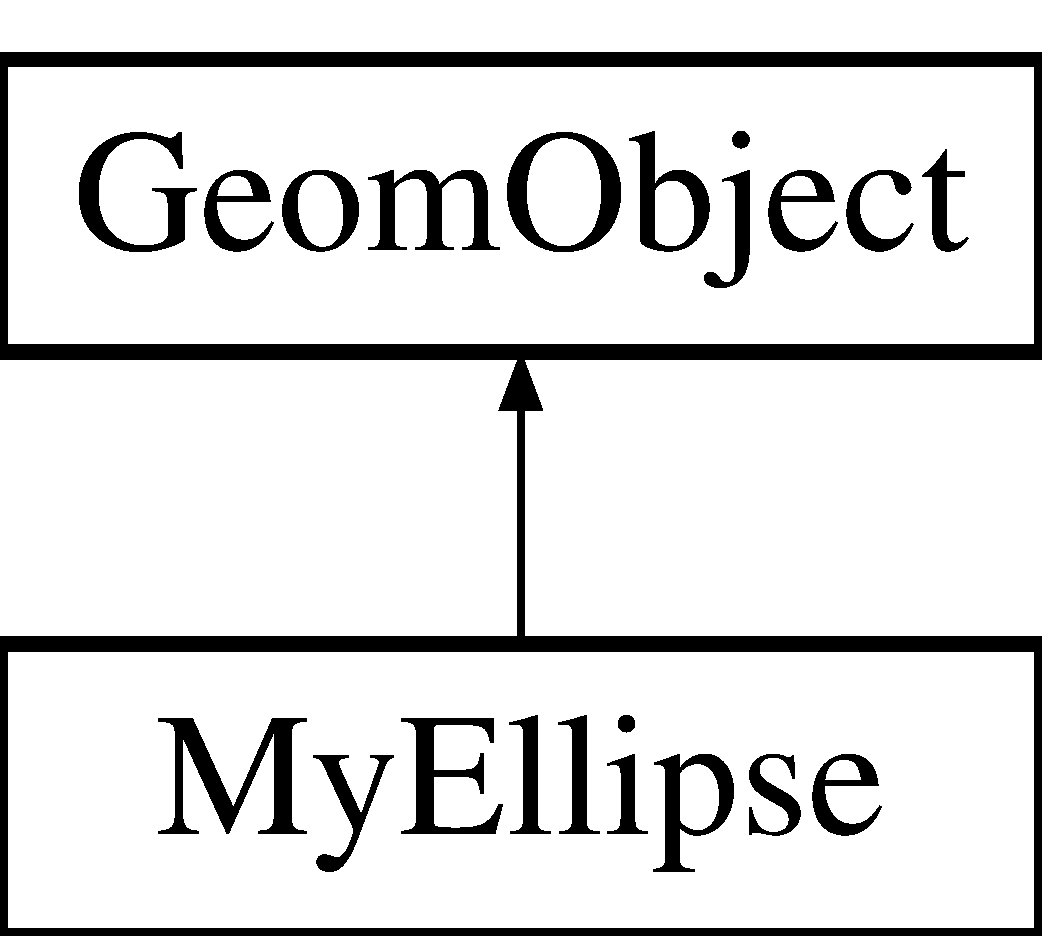
\includegraphics[height=2.000000cm]{classMyEllipse}
\end{center}
\end{figure}
\subsection*{Public Member Functions}
\begin{DoxyCompactItemize}
\item 
\hyperlink{classMyEllipse_a6d780f1f450d99e175842e88a3079069}{My\+Ellipse} (const double \&a, const double \&a\+\_\+hat, const double \&period, Time $\ast$time\+\_\+pt)
\begin{DoxyCompactList}\small\item\em Constructor\+: Pass initial x-\/half axis, amplitude of x-\/variation, period of oscillation and pointer to time object. \end{DoxyCompactList}\item 
virtual \hyperlink{classMyEllipse_ac2f2d3fb269c57fb26b4db6d9a0c7c05}{$\sim$\+My\+Ellipse} ()
\begin{DoxyCompactList}\small\item\em Destructor\+: Empty. \end{DoxyCompactList}\item 
void \hyperlink{classMyEllipse_a7b139a2f4564005773c83325f2414e3e}{position} (const Vector$<$ double $>$ \&xi, Vector$<$ double $>$ \&r) const
\begin{DoxyCompactList}\small\item\em Current position vector to material point at Lagrangian coordinate xi. \end{DoxyCompactList}\item 
void \hyperlink{classMyEllipse_a93f75bf33969037e35d779738a8493f5}{position} (const unsigned \&t, const Vector$<$ double $>$ \&xi, Vector$<$ double $>$ \&r) const
\begin{DoxyCompactList}\small\item\em Parametrised position on object\+: r(xi). Evaluated at previous time level. t=0\+: current time; t$>$0\+: previous time level. \end{DoxyCompactList}\end{DoxyCompactItemize}
\subsection*{Private Attributes}
\begin{DoxyCompactItemize}
\item 
double \hyperlink{classMyEllipse_aa2a0efd0a39f9d4fc307a6ff011682ed}{A}
\begin{DoxyCompactList}\small\item\em x-\/half axis \end{DoxyCompactList}\item 
double \hyperlink{classMyEllipse_a653e71cf296cdc86cc595d16f18004dd}{A\+\_\+hat}
\begin{DoxyCompactList}\small\item\em Amplitude of variation in x-\/half axis. \end{DoxyCompactList}\item 
double \hyperlink{classMyEllipse_ab098069ab23bbbd8f30b0da3523dc87f}{T}
\begin{DoxyCompactList}\small\item\em Period of oscillation. \end{DoxyCompactList}\item 
Time $\ast$ \hyperlink{classMyEllipse_abc1c4c863a599ce87bdff1abb9971953}{Time\+\_\+pt}
\begin{DoxyCompactList}\small\item\em Pointer to time object. \end{DoxyCompactList}\end{DoxyCompactItemize}


\subsection{Detailed Description}
Oscillating ellipse \[ x = (A + \widehat{A} \cos(2\pi t/T)) \cos(\xi) \] \[ y = \frac{\sin(\xi)}{A + \widehat{A} \cos(2\pi t/T)} \] Note that cross-\/sectional area is conserved. 

Definition at line 51 of file osc\+\_\+quarter\+\_\+ellipse.\+cc.



\subsection{Constructor \& Destructor Documentation}
\mbox{\Hypertarget{classMyEllipse_a6d780f1f450d99e175842e88a3079069}\label{classMyEllipse_a6d780f1f450d99e175842e88a3079069}} 
\index{My\+Ellipse@{My\+Ellipse}!My\+Ellipse@{My\+Ellipse}}
\index{My\+Ellipse@{My\+Ellipse}!My\+Ellipse@{My\+Ellipse}}
\subsubsection{\texorpdfstring{My\+Ellipse()}{MyEllipse()}}
{\footnotesize\ttfamily My\+Ellipse\+::\+My\+Ellipse (\begin{DoxyParamCaption}\item[{const double \&}]{a,  }\item[{const double \&}]{a\+\_\+hat,  }\item[{const double \&}]{period,  }\item[{Time $\ast$}]{time\+\_\+pt }\end{DoxyParamCaption})\hspace{0.3cm}{\ttfamily [inline]}}



Constructor\+: Pass initial x-\/half axis, amplitude of x-\/variation, period of oscillation and pointer to time object. 



Definition at line 58 of file osc\+\_\+quarter\+\_\+ellipse.\+cc.

\mbox{\Hypertarget{classMyEllipse_ac2f2d3fb269c57fb26b4db6d9a0c7c05}\label{classMyEllipse_ac2f2d3fb269c57fb26b4db6d9a0c7c05}} 
\index{My\+Ellipse@{My\+Ellipse}!````~My\+Ellipse@{$\sim$\+My\+Ellipse}}
\index{````~My\+Ellipse@{$\sim$\+My\+Ellipse}!My\+Ellipse@{My\+Ellipse}}
\subsubsection{\texorpdfstring{$\sim$\+My\+Ellipse()}{~MyEllipse()}}
{\footnotesize\ttfamily virtual My\+Ellipse\+::$\sim$\+My\+Ellipse (\begin{DoxyParamCaption}{ }\end{DoxyParamCaption})\hspace{0.3cm}{\ttfamily [inline]}, {\ttfamily [virtual]}}



Destructor\+: Empty. 



Definition at line 63 of file osc\+\_\+quarter\+\_\+ellipse.\+cc.



\subsection{Member Function Documentation}
\mbox{\Hypertarget{classMyEllipse_a7b139a2f4564005773c83325f2414e3e}\label{classMyEllipse_a7b139a2f4564005773c83325f2414e3e}} 
\index{My\+Ellipse@{My\+Ellipse}!position@{position}}
\index{position@{position}!My\+Ellipse@{My\+Ellipse}}
\subsubsection{\texorpdfstring{position()}{position()}\hspace{0.1cm}{\footnotesize\ttfamily [1/2]}}
{\footnotesize\ttfamily void My\+Ellipse\+::position (\begin{DoxyParamCaption}\item[{const Vector$<$ double $>$ \&}]{xi,  }\item[{Vector$<$ double $>$ \&}]{r }\end{DoxyParamCaption}) const\hspace{0.3cm}{\ttfamily [inline]}}



Current position vector to material point at Lagrangian coordinate xi. 



Definition at line 67 of file osc\+\_\+quarter\+\_\+ellipse.\+cc.



References Global\+\_\+\+Physical\+\_\+\+Variables\+::A, Global\+\_\+\+Physical\+\_\+\+Variables\+::\+A\+\_\+hat, and Global\+\_\+\+Physical\+\_\+\+Variables\+::T.

\mbox{\Hypertarget{classMyEllipse_a93f75bf33969037e35d779738a8493f5}\label{classMyEllipse_a93f75bf33969037e35d779738a8493f5}} 
\index{My\+Ellipse@{My\+Ellipse}!position@{position}}
\index{position@{position}!My\+Ellipse@{My\+Ellipse}}
\subsubsection{\texorpdfstring{position()}{position()}\hspace{0.1cm}{\footnotesize\ttfamily [2/2]}}
{\footnotesize\ttfamily void My\+Ellipse\+::position (\begin{DoxyParamCaption}\item[{const unsigned \&}]{t,  }\item[{const Vector$<$ double $>$ \&}]{xi,  }\item[{Vector$<$ double $>$ \&}]{r }\end{DoxyParamCaption}) const\hspace{0.3cm}{\ttfamily [inline]}}



Parametrised position on object\+: r(xi). Evaluated at previous time level. t=0\+: current time; t$>$0\+: previous time level. 



Definition at line 81 of file osc\+\_\+quarter\+\_\+ellipse.\+cc.



References Global\+\_\+\+Physical\+\_\+\+Variables\+::A, Global\+\_\+\+Physical\+\_\+\+Variables\+::\+A\+\_\+hat, and Global\+\_\+\+Physical\+\_\+\+Variables\+::T.



\subsection{Member Data Documentation}
\mbox{\Hypertarget{classMyEllipse_aa2a0efd0a39f9d4fc307a6ff011682ed}\label{classMyEllipse_aa2a0efd0a39f9d4fc307a6ff011682ed}} 
\index{My\+Ellipse@{My\+Ellipse}!A@{A}}
\index{A@{A}!My\+Ellipse@{My\+Ellipse}}
\subsubsection{\texorpdfstring{A}{A}}
{\footnotesize\ttfamily double My\+Ellipse\+::A\hspace{0.3cm}{\ttfamily [private]}}



x-\/half axis 



Definition at line 96 of file osc\+\_\+quarter\+\_\+ellipse.\+cc.

\mbox{\Hypertarget{classMyEllipse_a653e71cf296cdc86cc595d16f18004dd}\label{classMyEllipse_a653e71cf296cdc86cc595d16f18004dd}} 
\index{My\+Ellipse@{My\+Ellipse}!A\+\_\+hat@{A\+\_\+hat}}
\index{A\+\_\+hat@{A\+\_\+hat}!My\+Ellipse@{My\+Ellipse}}
\subsubsection{\texorpdfstring{A\+\_\+hat}{A\_hat}}
{\footnotesize\ttfamily double My\+Ellipse\+::\+A\+\_\+hat\hspace{0.3cm}{\ttfamily [private]}}



Amplitude of variation in x-\/half axis. 



Definition at line 99 of file osc\+\_\+quarter\+\_\+ellipse.\+cc.

\mbox{\Hypertarget{classMyEllipse_ab098069ab23bbbd8f30b0da3523dc87f}\label{classMyEllipse_ab098069ab23bbbd8f30b0da3523dc87f}} 
\index{My\+Ellipse@{My\+Ellipse}!T@{T}}
\index{T@{T}!My\+Ellipse@{My\+Ellipse}}
\subsubsection{\texorpdfstring{T}{T}}
{\footnotesize\ttfamily double My\+Ellipse\+::T\hspace{0.3cm}{\ttfamily [private]}}



Period of oscillation. 



Definition at line 102 of file osc\+\_\+quarter\+\_\+ellipse.\+cc.

\mbox{\Hypertarget{classMyEllipse_abc1c4c863a599ce87bdff1abb9971953}\label{classMyEllipse_abc1c4c863a599ce87bdff1abb9971953}} 
\index{My\+Ellipse@{My\+Ellipse}!Time\+\_\+pt@{Time\+\_\+pt}}
\index{Time\+\_\+pt@{Time\+\_\+pt}!My\+Ellipse@{My\+Ellipse}}
\subsubsection{\texorpdfstring{Time\+\_\+pt}{Time\_pt}}
{\footnotesize\ttfamily Time$\ast$ My\+Ellipse\+::\+Time\+\_\+pt\hspace{0.3cm}{\ttfamily [private]}}



Pointer to time object. 



Definition at line 105 of file osc\+\_\+quarter\+\_\+ellipse.\+cc.



The documentation for this class was generated from the following file\+:\begin{DoxyCompactItemize}
\item 
\hyperlink{osc__quarter__ellipse_8cc}{osc\+\_\+quarter\+\_\+ellipse.\+cc}\end{DoxyCompactItemize}

\hypertarget{classOscEllipseProblem}{}\section{Osc\+Ellipse\+Problem$<$ E\+L\+E\+M\+E\+NT, T\+I\+M\+E\+S\+T\+E\+P\+P\+ER $>$ Class Template Reference}
\label{classOscEllipseProblem}\index{Osc\+Ellipse\+Problem$<$ E\+L\+E\+M\+E\+N\+T, T\+I\+M\+E\+S\+T\+E\+P\+P\+E\+R $>$@{Osc\+Ellipse\+Problem$<$ E\+L\+E\+M\+E\+N\+T, T\+I\+M\+E\+S\+T\+E\+P\+P\+E\+R $>$}}


Navier-\/\+Stokes problem in an oscillating ellipse domain.  


Inheritance diagram for Osc\+Ellipse\+Problem$<$ E\+L\+E\+M\+E\+NT, T\+I\+M\+E\+S\+T\+E\+P\+P\+ER $>$\+:\begin{figure}[H]
\begin{center}
\leavevmode
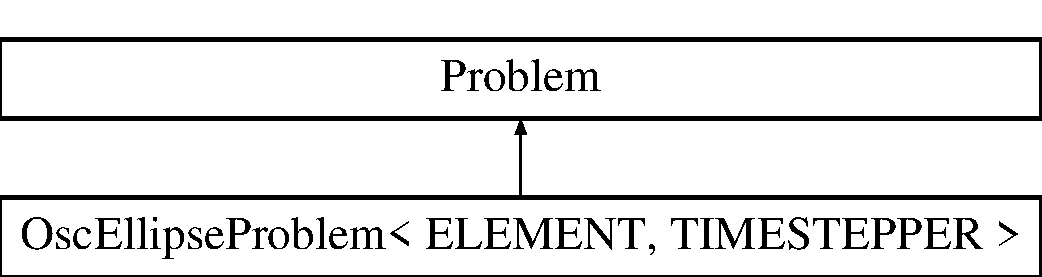
\includegraphics[height=2.000000cm]{classOscEllipseProblem}
\end{center}
\end{figure}
\subsection*{Public Member Functions}
\begin{DoxyCompactItemize}
\item 
\hyperlink{classOscEllipseProblem_aaa836937ec963921243fcb990f6fe538}{Osc\+Ellipse\+Problem} ()
\begin{DoxyCompactList}\small\item\em Constructor. \end{DoxyCompactList}\item 
\hyperlink{classOscEllipseProblem_a48a38acb7db1b394f7bfcd02e779b795}{$\sim$\+Osc\+Ellipse\+Problem} ()
\begin{DoxyCompactList}\small\item\em Destructor (empty) \end{DoxyCompactList}\item 
void \hyperlink{classOscEllipseProblem_a268e14b24e3ac922e7362bbb37ccde1f}{actions\+\_\+after\+\_\+newton\+\_\+solve} ()
\begin{DoxyCompactList}\small\item\em Update the problem specs after solve (empty) \end{DoxyCompactList}\item 
void \hyperlink{classOscEllipseProblem_a18bbd70aa8c140637637053a5f839c11}{actions\+\_\+before\+\_\+newton\+\_\+solve} ()
\begin{DoxyCompactList}\small\item\em Update problem specs before solve (empty) \end{DoxyCompactList}\item 
void \hyperlink{classOscEllipseProblem_a97c1b0056acbb9a6ec6157b6e7ad258a}{actions\+\_\+before\+\_\+adapt} ()
\begin{DoxyCompactList}\small\item\em Actions before adapt (empty) \end{DoxyCompactList}\item 
void \hyperlink{classOscEllipseProblem_a6044661f75986848484df2c04bfe7aab}{actions\+\_\+after\+\_\+adapt} ()
\begin{DoxyCompactList}\small\item\em Actions after adaptation, pin relevant pressures. \end{DoxyCompactList}\item 
void \hyperlink{classOscEllipseProblem_a7b12b4fdfcb46c3f00885f0a1f9965b3}{actions\+\_\+before\+\_\+implicit\+\_\+timestep} ()
\begin{DoxyCompactList}\small\item\em Update the problem specs before next timestep. \end{DoxyCompactList}\item 
void \hyperlink{classOscEllipseProblem_a80b50009a6aba4b6920c11b86b06f0f9}{actions\+\_\+after\+\_\+implicit\+\_\+timestep} ()
\begin{DoxyCompactList}\small\item\em Update the problem specs after timestep (empty) \end{DoxyCompactList}\item 
void \hyperlink{classOscEllipseProblem_afca2cc3e3e64ac764323f232cacc7e3b}{doc\+\_\+solution} (Doc\+Info \&doc\+\_\+info)
\begin{DoxyCompactList}\small\item\em Doc the solution. \end{DoxyCompactList}\item 
void \hyperlink{classOscEllipseProblem_ad0d879edbbd8b09b61e802ab66ef98a3}{unsteady\+\_\+run} (Doc\+Info \&doc\+\_\+info)
\begin{DoxyCompactList}\small\item\em Timestepping loop. \end{DoxyCompactList}\item 
void \hyperlink{classOscEllipseProblem_ae638f238a7b0e0acb5d6087b7363fe01}{set\+\_\+initial\+\_\+condition} ()
\begin{DoxyCompactList}\small\item\em Set initial condition. \end{DoxyCompactList}\end{DoxyCompactItemize}
\subsection*{Private Member Functions}
\begin{DoxyCompactItemize}
\item 
void \hyperlink{classOscEllipseProblem_a8b70831d1c25a40c814d5d92e77a1085}{fix\+\_\+pressure} (const unsigned \&e, const unsigned \&pdof, const double \&pvalue)
\begin{DoxyCompactList}\small\item\em Fix pressure in element e at pressure dof pdof and set to pvalue. \end{DoxyCompactList}\end{DoxyCompactItemize}
\subsection*{Private Attributes}
\begin{DoxyCompactItemize}
\item 
Geom\+Object $\ast$ \hyperlink{classOscEllipseProblem_a7d33f6345bf94cfe5165c4b9f2064ee6}{Wall\+\_\+pt}
\begin{DoxyCompactList}\small\item\em Pointer to Geom\+Object that specifies the domain bondary. \end{DoxyCompactList}\end{DoxyCompactItemize}


\subsection{Detailed Description}
\subsubsection*{template$<$class E\+L\+E\+M\+E\+NT, class T\+I\+M\+E\+S\+T\+E\+P\+P\+ER$>$\newline
class Osc\+Ellipse\+Problem$<$ E\+L\+E\+M\+E\+N\+T, T\+I\+M\+E\+S\+T\+E\+P\+P\+E\+R $>$}

Navier-\/\+Stokes problem in an oscillating ellipse domain. 

Definition at line 182 of file osc\+\_\+quarter\+\_\+ellipse.\+cc.



\subsection{Constructor \& Destructor Documentation}
\mbox{\Hypertarget{classOscEllipseProblem_aaa836937ec963921243fcb990f6fe538}\label{classOscEllipseProblem_aaa836937ec963921243fcb990f6fe538}} 
\index{Osc\+Ellipse\+Problem@{Osc\+Ellipse\+Problem}!Osc\+Ellipse\+Problem@{Osc\+Ellipse\+Problem}}
\index{Osc\+Ellipse\+Problem@{Osc\+Ellipse\+Problem}!Osc\+Ellipse\+Problem@{Osc\+Ellipse\+Problem}}
\subsubsection{\texorpdfstring{Osc\+Ellipse\+Problem()}{OscEllipseProblem()}}
{\footnotesize\ttfamily template$<$class E\+L\+E\+M\+E\+NT , class T\+I\+M\+E\+S\+T\+E\+P\+P\+ER $>$ \\
\hyperlink{classOscEllipseProblem}{Osc\+Ellipse\+Problem}$<$ E\+L\+E\+M\+E\+NT, T\+I\+M\+E\+S\+T\+E\+P\+P\+ER $>$\+::\hyperlink{classOscEllipseProblem}{Osc\+Ellipse\+Problem} (\begin{DoxyParamCaption}{ }\end{DoxyParamCaption})}



Constructor. 

Constructor for Navier-\/\+Stokes problem on an oscillating ellipse domain. 

Definition at line 273 of file osc\+\_\+quarter\+\_\+ellipse.\+cc.



References Global\+\_\+\+Physical\+\_\+\+Variables\+::A, Global\+\_\+\+Physical\+\_\+\+Variables\+::\+A\+\_\+hat, Global\+\_\+\+Physical\+\_\+\+Variables\+::\+Re, Global\+\_\+\+Physical\+\_\+\+Variables\+::\+Re\+St, and Global\+\_\+\+Physical\+\_\+\+Variables\+::T.

\mbox{\Hypertarget{classOscEllipseProblem_a48a38acb7db1b394f7bfcd02e779b795}\label{classOscEllipseProblem_a48a38acb7db1b394f7bfcd02e779b795}} 
\index{Osc\+Ellipse\+Problem@{Osc\+Ellipse\+Problem}!````~Osc\+Ellipse\+Problem@{$\sim$\+Osc\+Ellipse\+Problem}}
\index{````~Osc\+Ellipse\+Problem@{$\sim$\+Osc\+Ellipse\+Problem}!Osc\+Ellipse\+Problem@{Osc\+Ellipse\+Problem}}
\subsubsection{\texorpdfstring{$\sim$\+Osc\+Ellipse\+Problem()}{~OscEllipseProblem()}}
{\footnotesize\ttfamily template$<$class E\+L\+E\+M\+E\+NT, class T\+I\+M\+E\+S\+T\+E\+P\+P\+ER$>$ \\
\hyperlink{classOscEllipseProblem}{Osc\+Ellipse\+Problem}$<$ E\+L\+E\+M\+E\+NT, T\+I\+M\+E\+S\+T\+E\+P\+P\+ER $>$\+::$\sim$\hyperlink{classOscEllipseProblem}{Osc\+Ellipse\+Problem} (\begin{DoxyParamCaption}{ }\end{DoxyParamCaption})\hspace{0.3cm}{\ttfamily [inline]}}



Destructor (empty) 



Definition at line 191 of file osc\+\_\+quarter\+\_\+ellipse.\+cc.



\subsection{Member Function Documentation}
\mbox{\Hypertarget{classOscEllipseProblem_a6044661f75986848484df2c04bfe7aab}\label{classOscEllipseProblem_a6044661f75986848484df2c04bfe7aab}} 
\index{Osc\+Ellipse\+Problem@{Osc\+Ellipse\+Problem}!actions\+\_\+after\+\_\+adapt@{actions\+\_\+after\+\_\+adapt}}
\index{actions\+\_\+after\+\_\+adapt@{actions\+\_\+after\+\_\+adapt}!Osc\+Ellipse\+Problem@{Osc\+Ellipse\+Problem}}
\subsubsection{\texorpdfstring{actions\+\_\+after\+\_\+adapt()}{actions\_after\_adapt()}}
{\footnotesize\ttfamily template$<$class E\+L\+E\+M\+E\+NT, class T\+I\+M\+E\+S\+T\+E\+P\+P\+ER$>$ \\
void \hyperlink{classOscEllipseProblem}{Osc\+Ellipse\+Problem}$<$ E\+L\+E\+M\+E\+NT, T\+I\+M\+E\+S\+T\+E\+P\+P\+ER $>$\+::actions\+\_\+after\+\_\+adapt (\begin{DoxyParamCaption}{ }\end{DoxyParamCaption})\hspace{0.3cm}{\ttfamily [inline]}}



Actions after adaptation, pin relevant pressures. 



Definition at line 203 of file osc\+\_\+quarter\+\_\+ellipse.\+cc.

\mbox{\Hypertarget{classOscEllipseProblem_a80b50009a6aba4b6920c11b86b06f0f9}\label{classOscEllipseProblem_a80b50009a6aba4b6920c11b86b06f0f9}} 
\index{Osc\+Ellipse\+Problem@{Osc\+Ellipse\+Problem}!actions\+\_\+after\+\_\+implicit\+\_\+timestep@{actions\+\_\+after\+\_\+implicit\+\_\+timestep}}
\index{actions\+\_\+after\+\_\+implicit\+\_\+timestep@{actions\+\_\+after\+\_\+implicit\+\_\+timestep}!Osc\+Ellipse\+Problem@{Osc\+Ellipse\+Problem}}
\subsubsection{\texorpdfstring{actions\+\_\+after\+\_\+implicit\+\_\+timestep()}{actions\_after\_implicit\_timestep()}}
{\footnotesize\ttfamily template$<$class E\+L\+E\+M\+E\+NT, class T\+I\+M\+E\+S\+T\+E\+P\+P\+ER$>$ \\
void \hyperlink{classOscEllipseProblem}{Osc\+Ellipse\+Problem}$<$ E\+L\+E\+M\+E\+NT, T\+I\+M\+E\+S\+T\+E\+P\+P\+ER $>$\+::actions\+\_\+after\+\_\+implicit\+\_\+timestep (\begin{DoxyParamCaption}{ }\end{DoxyParamCaption})\hspace{0.3cm}{\ttfamily [inline]}}



Update the problem specs after timestep (empty) 



Definition at line 240 of file osc\+\_\+quarter\+\_\+ellipse.\+cc.

\mbox{\Hypertarget{classOscEllipseProblem_a268e14b24e3ac922e7362bbb37ccde1f}\label{classOscEllipseProblem_a268e14b24e3ac922e7362bbb37ccde1f}} 
\index{Osc\+Ellipse\+Problem@{Osc\+Ellipse\+Problem}!actions\+\_\+after\+\_\+newton\+\_\+solve@{actions\+\_\+after\+\_\+newton\+\_\+solve}}
\index{actions\+\_\+after\+\_\+newton\+\_\+solve@{actions\+\_\+after\+\_\+newton\+\_\+solve}!Osc\+Ellipse\+Problem@{Osc\+Ellipse\+Problem}}
\subsubsection{\texorpdfstring{actions\+\_\+after\+\_\+newton\+\_\+solve()}{actions\_after\_newton\_solve()}}
{\footnotesize\ttfamily template$<$class E\+L\+E\+M\+E\+NT, class T\+I\+M\+E\+S\+T\+E\+P\+P\+ER$>$ \\
void \hyperlink{classOscEllipseProblem}{Osc\+Ellipse\+Problem}$<$ E\+L\+E\+M\+E\+NT, T\+I\+M\+E\+S\+T\+E\+P\+P\+ER $>$\+::actions\+\_\+after\+\_\+newton\+\_\+solve (\begin{DoxyParamCaption}{ }\end{DoxyParamCaption})\hspace{0.3cm}{\ttfamily [inline]}}



Update the problem specs after solve (empty) 



Definition at line 194 of file osc\+\_\+quarter\+\_\+ellipse.\+cc.

\mbox{\Hypertarget{classOscEllipseProblem_a97c1b0056acbb9a6ec6157b6e7ad258a}\label{classOscEllipseProblem_a97c1b0056acbb9a6ec6157b6e7ad258a}} 
\index{Osc\+Ellipse\+Problem@{Osc\+Ellipse\+Problem}!actions\+\_\+before\+\_\+adapt@{actions\+\_\+before\+\_\+adapt}}
\index{actions\+\_\+before\+\_\+adapt@{actions\+\_\+before\+\_\+adapt}!Osc\+Ellipse\+Problem@{Osc\+Ellipse\+Problem}}
\subsubsection{\texorpdfstring{actions\+\_\+before\+\_\+adapt()}{actions\_before\_adapt()}}
{\footnotesize\ttfamily template$<$class E\+L\+E\+M\+E\+NT, class T\+I\+M\+E\+S\+T\+E\+P\+P\+ER$>$ \\
void \hyperlink{classOscEllipseProblem}{Osc\+Ellipse\+Problem}$<$ E\+L\+E\+M\+E\+NT, T\+I\+M\+E\+S\+T\+E\+P\+P\+ER $>$\+::actions\+\_\+before\+\_\+adapt (\begin{DoxyParamCaption}{ }\end{DoxyParamCaption})\hspace{0.3cm}{\ttfamily [inline]}}



Actions before adapt (empty) 



Definition at line 200 of file osc\+\_\+quarter\+\_\+ellipse.\+cc.

\mbox{\Hypertarget{classOscEllipseProblem_a7b12b4fdfcb46c3f00885f0a1f9965b3}\label{classOscEllipseProblem_a7b12b4fdfcb46c3f00885f0a1f9965b3}} 
\index{Osc\+Ellipse\+Problem@{Osc\+Ellipse\+Problem}!actions\+\_\+before\+\_\+implicit\+\_\+timestep@{actions\+\_\+before\+\_\+implicit\+\_\+timestep}}
\index{actions\+\_\+before\+\_\+implicit\+\_\+timestep@{actions\+\_\+before\+\_\+implicit\+\_\+timestep}!Osc\+Ellipse\+Problem@{Osc\+Ellipse\+Problem}}
\subsubsection{\texorpdfstring{actions\+\_\+before\+\_\+implicit\+\_\+timestep()}{actions\_before\_implicit\_timestep()}}
{\footnotesize\ttfamily template$<$class E\+L\+E\+M\+E\+NT, class T\+I\+M\+E\+S\+T\+E\+P\+P\+ER$>$ \\
void \hyperlink{classOscEllipseProblem}{Osc\+Ellipse\+Problem}$<$ E\+L\+E\+M\+E\+NT, T\+I\+M\+E\+S\+T\+E\+P\+P\+ER $>$\+::actions\+\_\+before\+\_\+implicit\+\_\+timestep (\begin{DoxyParamCaption}{ }\end{DoxyParamCaption})\hspace{0.3cm}{\ttfamily [inline]}}



Update the problem specs before next timestep. 



Definition at line 220 of file osc\+\_\+quarter\+\_\+ellipse.\+cc.

\mbox{\Hypertarget{classOscEllipseProblem_a18bbd70aa8c140637637053a5f839c11}\label{classOscEllipseProblem_a18bbd70aa8c140637637053a5f839c11}} 
\index{Osc\+Ellipse\+Problem@{Osc\+Ellipse\+Problem}!actions\+\_\+before\+\_\+newton\+\_\+solve@{actions\+\_\+before\+\_\+newton\+\_\+solve}}
\index{actions\+\_\+before\+\_\+newton\+\_\+solve@{actions\+\_\+before\+\_\+newton\+\_\+solve}!Osc\+Ellipse\+Problem@{Osc\+Ellipse\+Problem}}
\subsubsection{\texorpdfstring{actions\+\_\+before\+\_\+newton\+\_\+solve()}{actions\_before\_newton\_solve()}}
{\footnotesize\ttfamily template$<$class E\+L\+E\+M\+E\+NT, class T\+I\+M\+E\+S\+T\+E\+P\+P\+ER$>$ \\
void \hyperlink{classOscEllipseProblem}{Osc\+Ellipse\+Problem}$<$ E\+L\+E\+M\+E\+NT, T\+I\+M\+E\+S\+T\+E\+P\+P\+ER $>$\+::actions\+\_\+before\+\_\+newton\+\_\+solve (\begin{DoxyParamCaption}{ }\end{DoxyParamCaption})\hspace{0.3cm}{\ttfamily [inline]}}



Update problem specs before solve (empty) 



Definition at line 197 of file osc\+\_\+quarter\+\_\+ellipse.\+cc.

\mbox{\Hypertarget{classOscEllipseProblem_afca2cc3e3e64ac764323f232cacc7e3b}\label{classOscEllipseProblem_afca2cc3e3e64ac764323f232cacc7e3b}} 
\index{Osc\+Ellipse\+Problem@{Osc\+Ellipse\+Problem}!doc\+\_\+solution@{doc\+\_\+solution}}
\index{doc\+\_\+solution@{doc\+\_\+solution}!Osc\+Ellipse\+Problem@{Osc\+Ellipse\+Problem}}
\subsubsection{\texorpdfstring{doc\+\_\+solution()}{doc\_solution()}}
{\footnotesize\ttfamily template$<$class E\+L\+E\+M\+E\+NT , class T\+I\+M\+E\+S\+T\+E\+P\+P\+ER $>$ \\
void \hyperlink{classOscEllipseProblem}{Osc\+Ellipse\+Problem}$<$ E\+L\+E\+M\+E\+NT, T\+I\+M\+E\+S\+T\+E\+P\+P\+ER $>$\+::doc\+\_\+solution (\begin{DoxyParamCaption}\item[{Doc\+Info \&}]{doc\+\_\+info }\end{DoxyParamCaption})}



Doc the solution. 



Definition at line 470 of file osc\+\_\+quarter\+\_\+ellipse.\+cc.



References Global\+\_\+\+Physical\+\_\+\+Variables\+::get\+\_\+exact\+\_\+u().

\mbox{\Hypertarget{classOscEllipseProblem_a8b70831d1c25a40c814d5d92e77a1085}\label{classOscEllipseProblem_a8b70831d1c25a40c814d5d92e77a1085}} 
\index{Osc\+Ellipse\+Problem@{Osc\+Ellipse\+Problem}!fix\+\_\+pressure@{fix\+\_\+pressure}}
\index{fix\+\_\+pressure@{fix\+\_\+pressure}!Osc\+Ellipse\+Problem@{Osc\+Ellipse\+Problem}}
\subsubsection{\texorpdfstring{fix\+\_\+pressure()}{fix\_pressure()}}
{\footnotesize\ttfamily template$<$class E\+L\+E\+M\+E\+NT, class T\+I\+M\+E\+S\+T\+E\+P\+P\+ER$>$ \\
void \hyperlink{classOscEllipseProblem}{Osc\+Ellipse\+Problem}$<$ E\+L\+E\+M\+E\+NT, T\+I\+M\+E\+S\+T\+E\+P\+P\+ER $>$\+::fix\+\_\+pressure (\begin{DoxyParamCaption}\item[{const unsigned \&}]{e,  }\item[{const unsigned \&}]{pdof,  }\item[{const double \&}]{pvalue }\end{DoxyParamCaption})\hspace{0.3cm}{\ttfamily [inline]}, {\ttfamily [private]}}



Fix pressure in element e at pressure dof pdof and set to pvalue. 



Definition at line 254 of file osc\+\_\+quarter\+\_\+ellipse.\+cc.

\mbox{\Hypertarget{classOscEllipseProblem_ae638f238a7b0e0acb5d6087b7363fe01}\label{classOscEllipseProblem_ae638f238a7b0e0acb5d6087b7363fe01}} 
\index{Osc\+Ellipse\+Problem@{Osc\+Ellipse\+Problem}!set\+\_\+initial\+\_\+condition@{set\+\_\+initial\+\_\+condition}}
\index{set\+\_\+initial\+\_\+condition@{set\+\_\+initial\+\_\+condition}!Osc\+Ellipse\+Problem@{Osc\+Ellipse\+Problem}}
\subsubsection{\texorpdfstring{set\+\_\+initial\+\_\+condition()}{set\_initial\_condition()}}
{\footnotesize\ttfamily template$<$class E\+L\+E\+M\+E\+NT , class T\+I\+M\+E\+S\+T\+E\+P\+P\+ER $>$ \\
void \hyperlink{classOscEllipseProblem}{Osc\+Ellipse\+Problem}$<$ E\+L\+E\+M\+E\+NT, T\+I\+M\+E\+S\+T\+E\+P\+P\+ER $>$\+::set\+\_\+initial\+\_\+condition (\begin{DoxyParamCaption}{ }\end{DoxyParamCaption})}



Set initial condition. 

Set initial condition\+: Assign previous and current values from exact solution. 

Definition at line 396 of file osc\+\_\+quarter\+\_\+ellipse.\+cc.



References Global\+\_\+\+Physical\+\_\+\+Variables\+::get\+\_\+exact\+\_\+u().

\mbox{\Hypertarget{classOscEllipseProblem_ad0d879edbbd8b09b61e802ab66ef98a3}\label{classOscEllipseProblem_ad0d879edbbd8b09b61e802ab66ef98a3}} 
\index{Osc\+Ellipse\+Problem@{Osc\+Ellipse\+Problem}!unsteady\+\_\+run@{unsteady\+\_\+run}}
\index{unsteady\+\_\+run@{unsteady\+\_\+run}!Osc\+Ellipse\+Problem@{Osc\+Ellipse\+Problem}}
\subsubsection{\texorpdfstring{unsteady\+\_\+run()}{unsteady\_run()}}
{\footnotesize\ttfamily template$<$class E\+L\+E\+M\+E\+NT , class T\+I\+M\+E\+S\+T\+E\+P\+P\+ER $>$ \\
void \hyperlink{classOscEllipseProblem}{Osc\+Ellipse\+Problem}$<$ E\+L\+E\+M\+E\+NT, T\+I\+M\+E\+S\+T\+E\+P\+P\+ER $>$\+::unsteady\+\_\+run (\begin{DoxyParamCaption}\item[{Doc\+Info \&}]{doc\+\_\+info }\end{DoxyParamCaption})}



Timestepping loop. 

Unsteady run. 

Definition at line 562 of file osc\+\_\+quarter\+\_\+ellipse.\+cc.



Referenced by main().



\subsection{Member Data Documentation}
\mbox{\Hypertarget{classOscEllipseProblem_a7d33f6345bf94cfe5165c4b9f2064ee6}\label{classOscEllipseProblem_a7d33f6345bf94cfe5165c4b9f2064ee6}} 
\index{Osc\+Ellipse\+Problem@{Osc\+Ellipse\+Problem}!Wall\+\_\+pt@{Wall\+\_\+pt}}
\index{Wall\+\_\+pt@{Wall\+\_\+pt}!Osc\+Ellipse\+Problem@{Osc\+Ellipse\+Problem}}
\subsubsection{\texorpdfstring{Wall\+\_\+pt}{Wall\_pt}}
{\footnotesize\ttfamily template$<$class E\+L\+E\+M\+E\+NT, class T\+I\+M\+E\+S\+T\+E\+P\+P\+ER$>$ \\
Geom\+Object$\ast$ \hyperlink{classOscEllipseProblem}{Osc\+Ellipse\+Problem}$<$ E\+L\+E\+M\+E\+NT, T\+I\+M\+E\+S\+T\+E\+P\+P\+ER $>$\+::Wall\+\_\+pt\hspace{0.3cm}{\ttfamily [private]}}



Pointer to Geom\+Object that specifies the domain bondary. 



Definition at line 263 of file osc\+\_\+quarter\+\_\+ellipse.\+cc.



The documentation for this class was generated from the following file\+:\begin{DoxyCompactItemize}
\item 
\hyperlink{osc__quarter__ellipse_8cc}{osc\+\_\+quarter\+\_\+ellipse.\+cc}\end{DoxyCompactItemize}

\chapter{File Documentation}
\hypertarget{osc__ellipse_8txt__doxygenified_8h}{}\section{osc\+\_\+ellipse.\+txt\+\_\+doxygenified.\+h File Reference}
\label{osc__ellipse_8txt__doxygenified_8h}\index{osc\+\_\+ellipse.\+txt\+\_\+doxygenified.\+h@{osc\+\_\+ellipse.\+txt\+\_\+doxygenified.\+h}}

\hypertarget{osc__quarter__ellipse_8cc}{}\section{osc\+\_\+quarter\+\_\+ellipse.\+cc File Reference}
\label{osc__quarter__ellipse_8cc}\index{osc\+\_\+quarter\+\_\+ellipse.\+cc@{osc\+\_\+quarter\+\_\+ellipse.\+cc}}
\subsection*{Classes}
\begin{DoxyCompactItemize}
\item 
class \hyperlink{classMyEllipse}{My\+Ellipse}
\begin{DoxyCompactList}\small\item\em Oscillating ellipse \[ x = (A + \widehat{A} \cos(2\pi t/T)) \cos(\xi) \] \[ y = \frac{\sin(\xi)}{A + \widehat{A} \cos(2\pi t/T)} \] Note that cross-\/sectional area is conserved. \end{DoxyCompactList}\item 
class \hyperlink{classOscEllipseProblem}{Osc\+Ellipse\+Problem$<$ E\+L\+E\+M\+E\+N\+T, T\+I\+M\+E\+S\+T\+E\+P\+P\+E\+R $>$}
\begin{DoxyCompactList}\small\item\em Navier-\/\+Stokes problem in an oscillating ellipse domain. \end{DoxyCompactList}\end{DoxyCompactItemize}
\subsection*{Namespaces}
\begin{DoxyCompactItemize}
\item 
 \hyperlink{namespaceGlobal__Physical__Variables}{Global\+\_\+\+Physical\+\_\+\+Variables}
\begin{DoxyCompactList}\small\item\em Namepspace for global parameters. \end{DoxyCompactList}\end{DoxyCompactItemize}
\subsection*{Functions}
\begin{DoxyCompactItemize}
\item 
void \hyperlink{namespaceGlobal__Physical__Variables_af29d0fbf7264555610176a1fc931591a}{Global\+\_\+\+Physical\+\_\+\+Variables\+::get\+\_\+exact\+\_\+u} (const double \&t, const Vector$<$ double $>$ \&x, Vector$<$ double $>$ \&u)
\begin{DoxyCompactList}\small\item\em Exact solution of the problem as a vector containing u,v,p. \end{DoxyCompactList}\item 
int \hyperlink{osc__quarter__ellipse_8cc_a0ddf1224851353fc92bfbff6f499fa97}{main} (int argc, char $\ast$argv\mbox{[}$\,$\mbox{]})
\end{DoxyCompactItemize}
\subsection*{Variables}
\begin{DoxyCompactItemize}
\item 
double \hyperlink{namespaceGlobal__Physical__Variables_ab814e627d2eb5bc50318879d19ab16b9}{Global\+\_\+\+Physical\+\_\+\+Variables\+::\+Re} =100.\+0
\begin{DoxyCompactList}\small\item\em Reynolds number. \end{DoxyCompactList}\item 
double \hyperlink{namespaceGlobal__Physical__Variables_a085ee4bf968ffdd01a41b8c41864f907}{Global\+\_\+\+Physical\+\_\+\+Variables\+::\+Re\+St} =100.\+0
\begin{DoxyCompactList}\small\item\em Womersley = Reynolds times Strouhal. \end{DoxyCompactList}\item 
double \hyperlink{namespaceGlobal__Physical__Variables_a4894f9a3a9cbf84f00d0719f2841e624}{Global\+\_\+\+Physical\+\_\+\+Variables\+::A} =1.\+0
\begin{DoxyCompactList}\small\item\em x-\/\+Half axis length \end{DoxyCompactList}\item 
double \hyperlink{namespaceGlobal__Physical__Variables_a11d1e77201d6b8c250c4c9396fc5ad06}{Global\+\_\+\+Physical\+\_\+\+Variables\+::\+A\+\_\+hat} =0.\+1
\begin{DoxyCompactList}\small\item\em x-\/\+Half axis amplitude \end{DoxyCompactList}\item 
double \hyperlink{namespaceGlobal__Physical__Variables_a1a806ee7c4d04d6afaba1d24d94dceea}{Global\+\_\+\+Physical\+\_\+\+Variables\+::T} =1.\+0
\begin{DoxyCompactList}\small\item\em Period of oscillations. \end{DoxyCompactList}\end{DoxyCompactItemize}


\subsection{Function Documentation}
\mbox{\Hypertarget{osc__quarter__ellipse_8cc_a0ddf1224851353fc92bfbff6f499fa97}\label{osc__quarter__ellipse_8cc_a0ddf1224851353fc92bfbff6f499fa97}} 
\index{osc\+\_\+quarter\+\_\+ellipse.\+cc@{osc\+\_\+quarter\+\_\+ellipse.\+cc}!main@{main}}
\index{main@{main}!osc\+\_\+quarter\+\_\+ellipse.\+cc@{osc\+\_\+quarter\+\_\+ellipse.\+cc}}
\subsubsection{\texorpdfstring{main()}{main()}}
{\footnotesize\ttfamily int main (\begin{DoxyParamCaption}\item[{int}]{argc,  }\item[{char $\ast$}]{argv\mbox{[}$\,$\mbox{]} }\end{DoxyParamCaption})}

Driver code for unsteady Navier-\/\+Stokes flow, driven by oscillating ellipse. If the code is executed with command line arguments, a validation run is performed. 

Definition at line 628 of file osc\+\_\+quarter\+\_\+ellipse.\+cc.



References Osc\+Ellipse\+Problem$<$ E\+L\+E\+M\+E\+N\+T, T\+I\+M\+E\+S\+T\+E\+P\+P\+E\+R $>$\+::unsteady\+\_\+run().


%--- End generated contents ---

% Index
\backmatter
\newpage
\phantomsection
\clearemptydoublepage
\addcontentsline{toc}{chapter}{Index}
\printindex

\end{document}
